%%%%%%%%%%%%%%%%%%%%%%%%%%%%%%%%%%%%%%%%%%%%%%%%%%%%%%%%%%%%%%%%%%%%%%
% How to use writeLaTeX: 
%
% You edit the source code here on the left, and the preview on the
% right shows you the result within a few seconds.
%
% Bookmark this page and share the URL with your co-authors. They can
% edit at the same time!
%
% You can upload figures, bibliographies, custom classes and
% styles using the files menu.
%
%%%%%%%%%%%%%%%%%%%%%%%%%%%%%%%%%%%%%%%%%%%%%%%%%%%%%%%%%%%%%%%%%%%%%%

\documentclass[12pt]{article}

\usepackage{sbc-template}

\usepackage{graphicx,url}

\usepackage[brazil]{babel}   
\usepackage[utf8]{inputenc}  

     
\sloppy

\title{Avaliação da efetividade de radares em rodovias federais da região Sul do Brasil}

\author{ Adriano Pertile\inst{1}, José A. Cidral\inst{2}, Muriel B. P. Guarezi\inst{3} }

\address{
Universidade Federal de Santa Catarina (UFSC) 
-- Joinville -- SC -- Brasil
\nextinstitute
Universidade Federal de Santa Catarina (UFSC) 
-- Joinville -- SC -- Brasil
\nextinstitute
Universidade Federal de Santa Catarina (UFSC) 
-- Joinville -- SC -- Brasil 
  \email{adriano.pertile.97@gmail.com}
  \email{jose.acidral@gmail.com}
  \email{muriel.guarezi1@gmail.com}
}

\begin{document} 

\maketitle

\begin{abstract}
  This meta-paper describes the style to be used in articles and short papers
  for SBC conferences. For papers in English, you should add just an abstract
  while for the papers in Portuguese, we also ask for an abstract in
  Portuguese (``resumo''). In both cases, abstracts should not have more than
  10 lines and must be in the first page of the paper.
\end{abstract}
     
\begin{resumo} 
  Este meta-artigo descreve o estilo a ser usado na confecção de artigos e
  resumos de artigos para publicação nos anais das conferências organizadas
  pela SBC. É solicitada a escrita de resumo e abstract apenas para os artigos
  escritos em português. Artigos em inglês deverão apresentar apenas abstract.
  Nos dois casos, o autor deve tomar cuidado para que o resumo (e o abstract)
  não ultrapassem 10 linhas cada, sendo que ambos devem estar na primeira
  página do artigo.
\end{resumo}

%%%%%%%%%%%%%%%%%%%%%%%%%%%%%%%%%%%%%%%%%%%%%%%%%%%%%%%%%%%%%%%%%%%%%%
\section{Introdução}
%%%%%%%%%%%%%%%%%%%%%%%%%%%%%%%%%%%%%%%%%%%%%%%%%%%%%%%%%%%%%%%%%%%%%%
A segurança viária representa um desafio de saúde pública global, com os acidentes de trânsito sendo responsáveis por 1,19 milhão de óbitos anuais em todo o mundo \cite{who2023}. 
No Brasil, os custos decorrentes de acidentes em rodovias e áreas urbanas alcançam dezenas de bilhões de reais anualmente, impactando os sistemas de saúde, previdenciário e a produtividade nacional \cite{ipea2020}. 

A Região Sul, um dos corredores logísticos do país, registrou 3.809 acidentes com vítimas fatais em rodovias federais no período de 2022 ao início de 2025 \cite{PRF_Dados_Abertos}, além de 52.603 acidentes com vítimas feridas (Figura \ref{fig:acidentes_22a25}.

\begin{figure}[!htb]
\centering
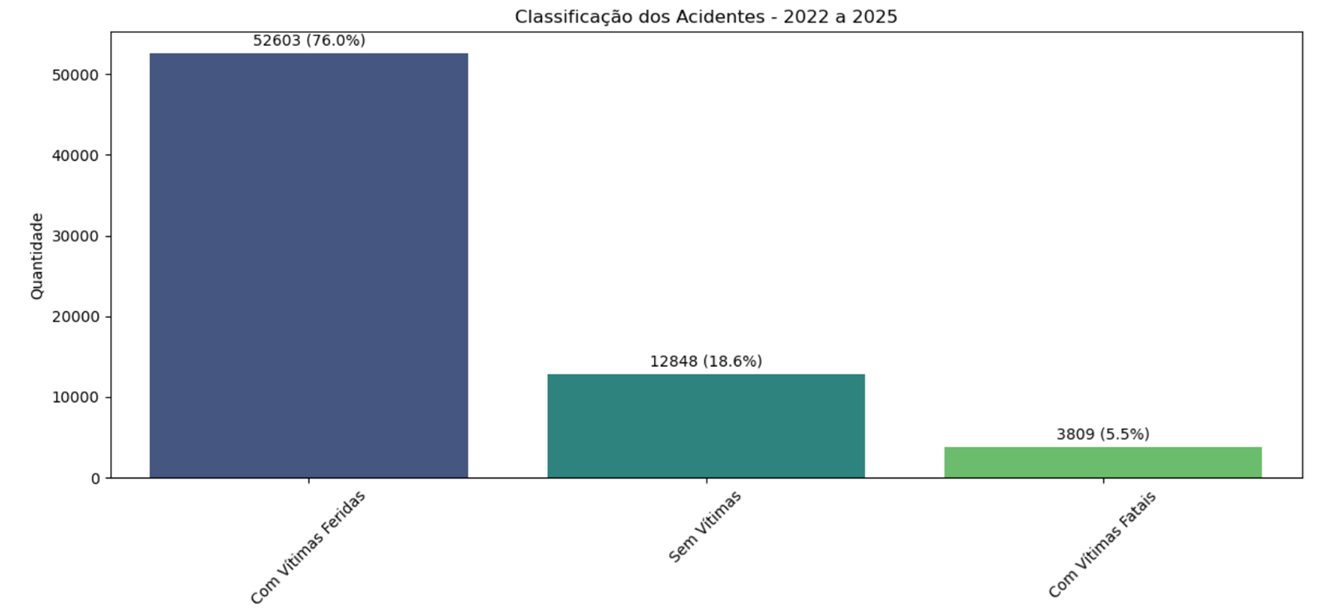
\includegraphics[width=1\textwidth]{figures/0/acidentes_22a25.png}
\caption{Dados de \cite{PRF_Dados_Abertos}.}
\label{fig:acidentes_22a25}
\end{figure}

A escolha da região como objeto de estudo fundamenta-se na densidade infraestrutural da região, possuindo a maior malha rodoviária federal pavimentada do país, com extensão de 20,5 km a cada mil quilômetros quadrados de área \cite{cnt2023}. A Figura \ref{fig:malhaRodoviaria_Regiao} apresenta um comparativo da densidade de rodovias pavimentadas por região do Brasil, no ano de 2024.
\begin{figure}[!htb]
\centering
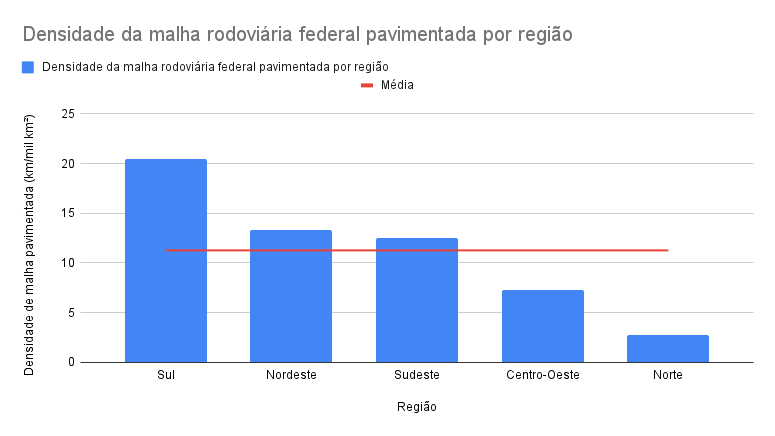
\includegraphics[width=1\textwidth]{figures/0/malhaRodoviaria_porRegiao.png}
\caption{Adaptado de \cite{cnt2023}.}
\label{fig:malhaRodoviaria_Regiao}
\end{figure}

Essa infraestrutura serve a uma área que corresponde a apenas 7\% do território nacional, mas que abriga 14,7\% da população brasileira, sendo responsável por aproximadamente 17\% do Produto Interno Bruto (PIB) do país \cite{ibge_pib_sul}.
A combinação da infraestrutura e atividade econômica da região, dada a densidade, eleva o risco de acidentes viários. 
Portanto, a análise desta região não apenas aborda um problema local, mas também gera percepções aplicáveis a outros corredores logísticos do país.

A literatura científica estabelece uma correlação direta e exponencial entre velocidade e risco. 
Estudos e revisões da área demonstram que um aumento de 1\% na velocidade média de um veículo pode resultar em um aumento de até 4\% na incidência de acidentes fatais \cite{aarts2006, hauer2009}. 
Nesse contexto, a fiscalização eletrônica por meio de radares consolidou-se como uma política pública baseada em evidências. 
Uma revisão sistemática da Cochrane Collaboration concluiu que a instalação de câmeras de velocidade está associada a reduções que podem variar de 11\% a 44\% nos acidentes com mortos e feridos graves nas imediações dos equipamentos \cite{wilson2010}.

Apesar da eficácia comprovada da fiscalização, a eficiência da política depende da alocação espacial dos equipamentos. 
A instalação de radares em locais de baixo risco ou com baixa adesão aos limites de velocidade pode não gerar o retorno esperado em termos de vidas salvas, deixando de otimizar recursos públicos \cite{kweon2011}. 

%%% Inserir mais estudos, artigos semelhantes, algo nesse sentido

Embora existam estudos internacionais sobre a otimização de radares, identifica-se uma lacuna na aplicação de uma abordagem metodológica integrada que utilize dados pós-pandêmicos recentes para a malha rodoviária federal brasileira. 
O diferencial deste trabalho reside na combinação de múltiplas técnicas de Ciência de Dados: 
\begin{itemize}
    \item A aplicação de estatística espacial, via Índice de Moran, para identificar pontos e clusters de alta sinistralidade estatisticamente relevantes;
    \item A quantificação da cobertura da fiscalização atual por meio de análises de buffer para identificar pontos com fiscalização insuficiente; 
    \item O desenvolvimento de um modelo preditivo para identificar os fatores mais críticos associados à gravidade dos acidentes. 
\end{itemize}

O presente estudo propõe-se a preencher essa lacuna por meio de uma análise quantitativa e geoespacial, partindo da premissa de que a análise de dados históricos de acidentes e infrações combinada com técnicas de estatística e modelos de aprendizado de máquina, permite identificar com maior precisão os pontos críticos da malha rodoviária.
Desta forma, o objetivo geral do trabalho é desenvolver um modelo data-driven para avaliar a disposição atual e indicar locais estratégicos para a instalação de novos radares nas rodovias federais dos estados do Paraná, Santa Catarina e Rio Grande do Sul. 
Para alcançar este fim, foram definidos os seguintes objetivos específicos:

\begin{itemize}
    \item Analisar o perfil e a distribuição de acidentes e infrações nas rodovias federais da região Sul, por meio de dados abertos do período pós-pandêmico, com enfoque nos acidentes com vítimas fatais envolvendo o excesso de velocidade, ou que poderiam ser mitigados pela instalação de radares;

    % \item Identificar as principais causas e características dos acidentes, com especial atenção àqueles de maior severidade;
    
    \item Aplicar métodos de análise de padrões de pontos, como o Índice de Moran, para detectar a presença de autocorrelação espacial e identificar clusters de alta sinistralidade;
    
    \item Avaliar a relação entre a localização da malha de radares existente e a concentração de acidentes, analisando a efetividade de sua cobertura espacial;
    
    % \item Propor uma metodologia para hierarquizar e indicar pontos prioritários para a instalação de novos equipamentos de fiscalização, fundamentada nos padrões identificados.
\end{itemize}

Este artigo está estruturado em cinco seções. 
Após esta introdução, a Seção 2 apresenta uma revisão dos trabalhos relacionados, discutindo abordagens metodológicas para análise de acidentes e otimização da localização de radares. 
A Seção 3 detalha a metodologia empregada, incluindo a descrição das fontes de dados e as técnicas de análise estatística e geoespacial. 
A Seção 4 apresenta e discute os resultados obtidos e, por fim, a Seção 5 sumariza as conclusões do estudo, aponta suas limitações e sugere direções para pesquisas futuras.

%%%%%%%%%%%%%%%%%%%%%%%%%%%%%%%%%%%%%%%%%%%%%%%%%%%%%%%%%%%%%%%%%%%%%%
\section{Trabalhos relacionados}
%%%%%%%%%%%%%%%%%%%%%%%%%%%%%%%%%%%%%%%%%%%%%%%%%%%%%%%%%%%%%%%%%%%%%%

Esta seção revisa alguns trabalhos pertinentes produzidos na última década, empregando uma estratégia de busca com filtros avançados nas bases de dados Scopus e o Portal de Periódicos da CAPES. 
A pesquisa resultou ao todo em 11 publicação, das quais sete foram selecionadas para estudo após análise qualitativa dos títulos. A análise priorizou produções com maior similaridade à metodologia do trabalho, ao contexto da região Sul e às aplicações de Ciência de Dados na segurança viária.
Os termos de busca e a combinação lógica utilizados foram: 
\begin{verbatim}
    ("ciência de dados" OR "análise espacial" OR "geopro-
    cessamento") AND ("segurança viária" OR "acidentes de
    trânsito") AND ("rodovias federais" OR "rodovias") 
    AND "Brasil"
\end{verbatim}

\cite{santana2024} investigou a distribuição espacial de acidentes urbanos em Arapiraca (AL), utilizando o Índice de Moran Global e Local como ferramenta estatística. Os dados foram agregados por bairros e a análise buscou identificar clusters de acidentes. Um achado relevante foi que o Moran Global não se mostrou estatisticamente significativo, com valor de 0,59, indicando a ausência de autocorrelação espacial na agregação por bairro.

\cite{santos2020} teve como objetivo identificar hotspots de acidentes nas rodovias federais de Goiás utilizando dados da PRF de 2014 a 2019, via Estimação de Densidade Kernel (KDE). O método permitiu visualizar os trechos com maior densidade de ocorrências, em pontos de interseção e conexões entre cidades.
% "Diferentemente de estudos que se baseiam na densidade visual (KDE), como o de Santos et al. (2020), nossa abordagem valida estatisticamente os clusters encontrados".

\cite{carmo2019} teve como enfoque o estudo da segurança nos trechos urbanos de rodovias federais na Região Sul. Os autores concluiram que esses segmentos estão entre os mais perigosos do país, alta sinistralidade mesmo com boas condições da via.
% mesmo com uma infraestrutura de rodovias bem classificadas pela CNT.
% dados da PRF e da CNT entre 2010 e 2014
% alta sinistralidade mesmo com boas condições da via;

\cite{moraisneto2012} analisou dados de mortalidade entre 2000 e 2010 e identificou os principais aglomerados de risco do país, com a identificação de um cluster de alto risco persistente e em expansão composto majoritariamente por municípios do Paraná e Santa Catarina.
% Fornece um contexto histórico e em escala nacional que corrobora à importância da pesquisa. 
% Ele prova que a Região Sul é um hotspot crônico de mortalidade no trânsito há mais de uma década. 
% Usar esse artigo na introdução para afirmar que o nosso trabalho investiga as políticas de mitigação atuais (alocação de radares) em um problema de longa data e de relevância nacional.

\cite{deona2021} discute a aplicação de \textit{data mining}, estatística, aprendizado de máquina à segurança viária. O artigo menciona a análise de clusters, modelos de classificação como árvores de decisão, e a importância da qualidade dos dados.
% Citá-lo para afirmar que a metodologia de análise de clusters, modelos de árvore de decisão e o uso de múltiplas fontes de dados está alinhada com as melhores práticas e o estado da arte internacional em Ciência de Dados para segurança viária.

\cite{nitsche2022} foca no desenvolvimento de Funções de Desempenho de Segurança (SPFs) para rodovias federais brasileiras, incluindo trechos em Santa Catarina e Paraná. SPFs são modelos estatísticos que preveem o número de acidentes com base em características da via e no volume de tráfego.
% previsão de acidentes com base na geometria e no fluxo da via.
% É um excelente artigo para citar em "Trabalhos Futuros", sugerindo que os clusters de acidentes poderiam ser enriquecidos com a análise de SPFs para entender melhor as causas ligadas à infraestrutura.

\cite{pinheiro2020} analisa a distribuição espacial da mortalidade de mulheres em acidentes de motocicleta em municipal nd Brasil, usando o estimador bayesiano empírico.
O artigo demonstrou como a análise espacial pode revelar dinâmicas regionais distintas para diferentes perfis de vítimas. 
% Você pode citá-lo para argumentar que, enquanto estudos focados em subgrupos são importantes, uma análise mais ampla como a sua é necessária para orientar políticas de fiscalização de caráter geral, como a instalação de radares.

%%%%%%%%%%%%%%%%%%%%%%%%%%%%%%%%%%%%%%%%%%%%%%%%%%%%%%%%%%%%%%%%%%%%%%
\section{Metodologia}
%%%%%%%%%%%%%%%%%%%%%%%%%%%%%%%%%%%%%%%%%%%%%%%%%%%%%%%%%%%%%%%%%%%%%%
Em um processo de aprendizagem, é necessário percorrer determinadas etapas antes que se possa afirmar que um novo conhecimento foi, de fato, adquirido. Nesse contexto, destaca-se o processo de Descoberta de Conhecimento em Bases de Dados (KDD – Knowledge Discovery in Databases), composto por nove etapas interativas.

A primeira etapa consiste no entendimento dos objetivos do projeto, estabelecendo seus limites e diretrizes. No caso em questão, o projeto tem como foco a identificação e indicação dos locais mais adequados para a instalação de radares, a partir da análise do histórico de acidentes e infrações.

A segunda etapa refere-se à seleção dos dados. Para os dados de acidentes e infrações, foram utilizados os dados abertos disponibilizados pela Polícia Rodoviária Federal (PRF), considerando registros a partir de 2022. No caso dos radares, recorreu-se a duas bases distintas: a da Agência Nacional de Transportes Terrestres (ANTT), que contempla os equipamentos instalados em rodovias federais concessionadas, e a do Departamento Nacional de Infraestrutura de Transportes (DNIT), referente às rodovias federais sob administração direta do governo. Além disso, como forma de complementar as informações sobre os radares, foram consultados o Google Street View e o Portal de Serviços do Inmetro nos estados, especialmente para obtenção dos dados relacionados à ativação dos equipamentos. Além disso foi utilizado os shapefiles dos municípios, disponibilizados pelo IBGE.

A terceira etapa corresponde ao pré-processamento e à integração dos dados. Nesse momento, os registros de acidentes foram filtrados de forma a considerar apenas aqueles em que a velocidade esteve diretamente associada à causa do evento. Para identificar essas causas, inicialmente foram extraídos os valores únicos presentes no conjunto de dados. Em seguida, esses valores foram submetidos a um prompt na LLM da OpenAI, a fim de obter uma lista das causas de acidentes que poderiam ser evitadas com a instalação de radares. Como resultado, foram definidas as seguintes causas: "Velocidade Incompatível", "Participar de racha", "Condutor deixou de manter distância do veículo da frente", "Reação tardia ou ineficiente do condutor", "Transitar na contramão", "Ultrapassagem Indevida", "Frear bruscamente", "Condutor usando celular", "Transitar no acostamento", "Transitar no Acostamento".

Nesta etapa, também foi realizada a coleta das prováveis datas de instalação dos radares. Para a base de dados da ANTT, não havia informações que permitissem identificar individualmente cada radar (como número de série). Dessa forma, utilizou-se o Google Street View, explorando as coordenadas disponibilizadas no arquivo e analisando as datas das imagens capturadas naquele ponto, a fim de estimar a instalação dos equipamentos. Já na base de dados do DNIT, cada radar possui um identificador único, permitindo consultar o Portal de Serviços do Inmetro nos estados para verificar tanto as manutenções quanto a data de instalação dos radares. As informações obtidas foram incorporadas ao dataset em duas novas colunas: uma contendo o mês de instalação e outra, o ano de instalação.

Na etapa de transformação, as colunas de latitude e longitude, presentes tanto no conjunto de dados de acidentes quanto no de radares, foram convertidas para valores numéricos, além da exclusão dos registros com dados ausentes. De acordo com a finalidade da análise, essas variáveis geográficas foram transformadas para diferentes sistemas de referência de coordenadas (CRS). Utilizou-se o EPSG:4326 quando a representação em graus decimais era necessária e o EPSG:31982 nos casos em que se demandavam cálculos de distância, uma vez que este sistema retorna medidas em metros. Os shapefiles dos municípios também foram padronizados para essas mesmas formatações, garantindo consistência na integração e análise espacial dos dados, como pode ser observado na Figura ~\ref{fig:exampleFig2}.

\begin{figure}[!htb]
\centering
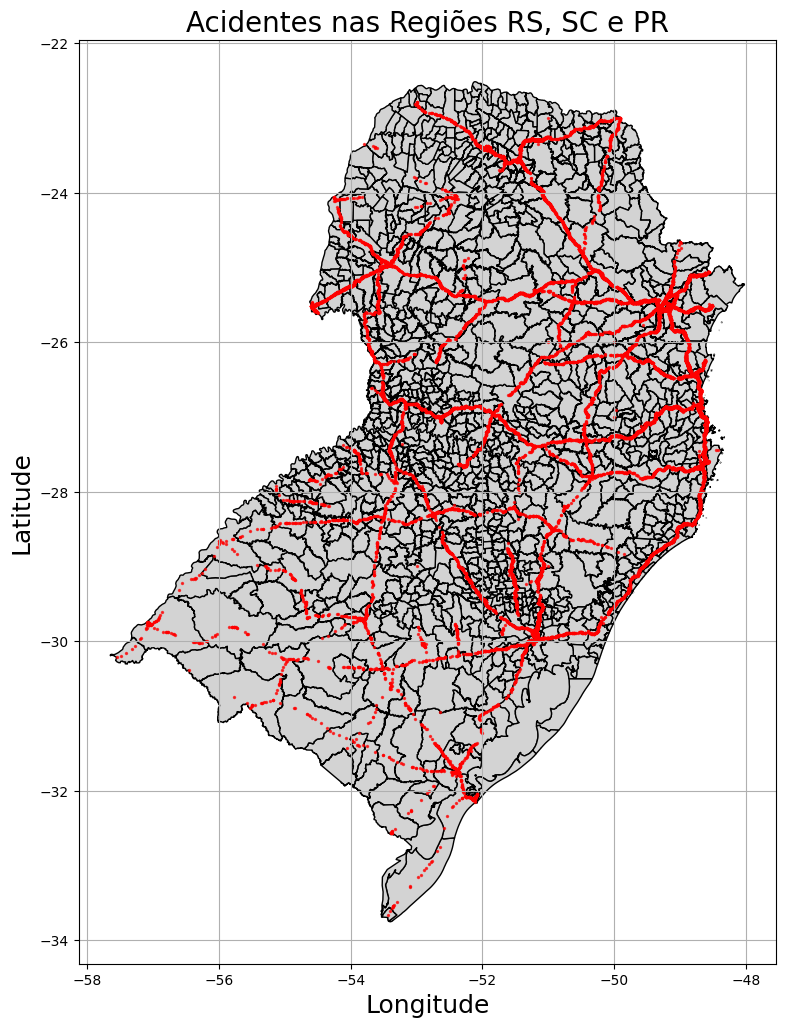
\includegraphics[width=.5\textwidth]{figures/2 - abordagem visualizacao/2 - acidentes regioes.png}
\caption{Acidentes em cada município}
\label{fig:exampleFig2}
\end{figure}

Para saber a quantidade de acidentes por cidade foi realizado um "join espacial" das cidades presentes dentro do shapefile com os acidentes, criando uma nova coluna com o número de acidentes. Com essa informação foi possível separar em clusters as cidades com a quantidade de acidentes presentes nelas, conforme a Figura ~\ref{fig:exampleFig3}.

\begin{figure}[!htb]
\centering
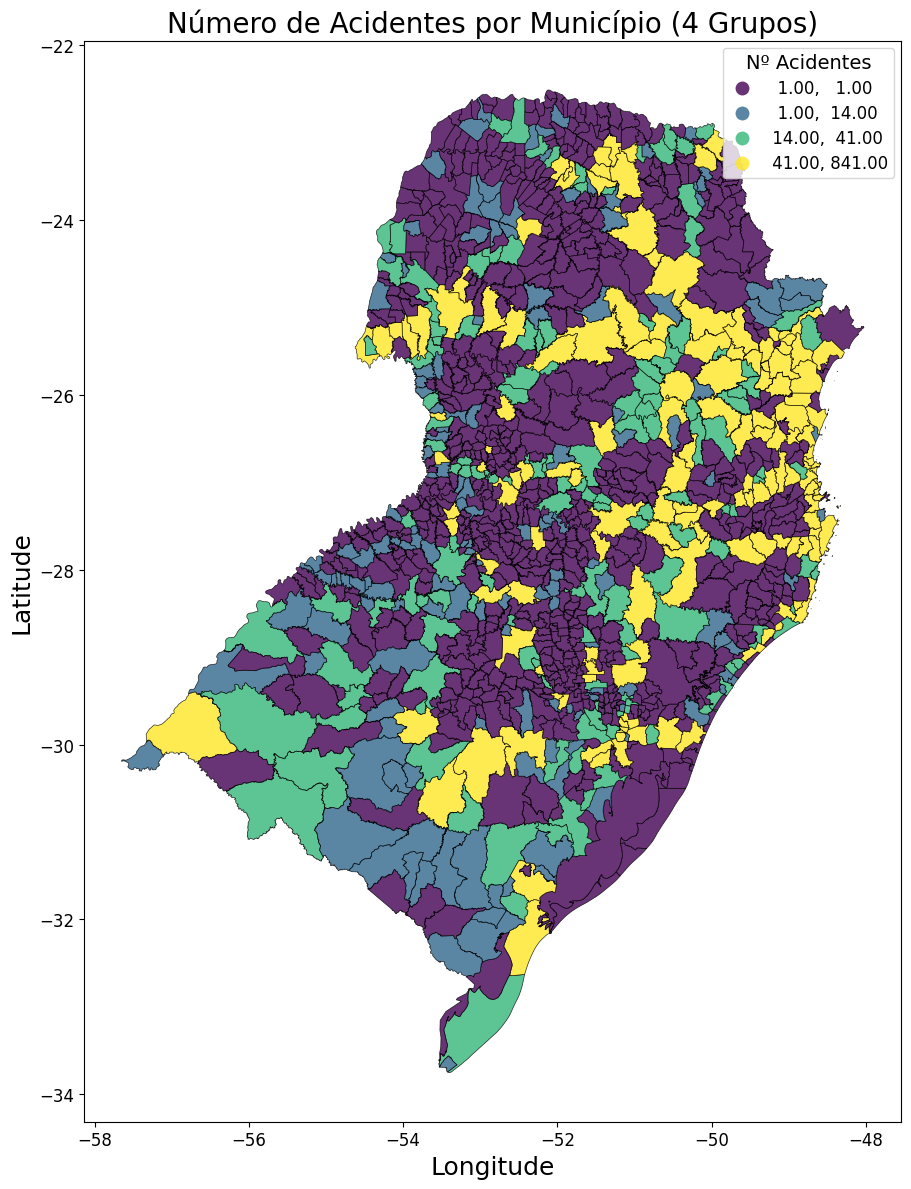
\includegraphics[width=.5\textwidth]{figures/2 - abordagem visualizacao/3 - agrupamento acidentes.png}
\caption{Número de acidentes por município}
\label{fig:exampleFig3}
\end{figure}

A próxima etapa foi a definição da matriz de vizinhança do dataset das cidades. Por exemplo, o vetor pode corresponder a observações de uma determinada variável
observada para cada município brasileiro, ou corresponder a observações de uma
variável para cada setor censitário na cidade de São Paulo. Neste caso, o elemento $W_{i,j}$
da matriz W assume valor $W_{i,j}$ = 1, caso os polígonos i e j sejam vizinhos, e $W_{i,j}$ = 0,
caso i e j não sejam vizinhos \cite{carvalho2010}. Existem algumas possibilidades diferentes de tipos de vizinhança, para este projeto foi utilizada a do tipo \textit{queen}, que representa um vizinho com pelo menos um vértice em comum.

Com a matriz W, é necessária a realização da sua normalização. A matriz normalizada $W_{n}$
é construída a partir da matriz W original (não normalizada), dividindo-se todos os
elementos de cada linha W de pela soma da linha \cite{carvalho2010}.

Utilizando a matriz de vizinhança e o dataset de acidentes por cidades é possível calcular índice de correlação espacial de Moran.  Esta estatística pode ser aplicada à variável $y_{i}$ diretamente, ou aos resíduos da regressão de $y_{i}$ versus um conjunto de variáveis explicativas \cite{carvalho2010}. Com essas duas informações é possível também calcular o índice de Moran local, com ele, é medido a associação entre a variável de interesse da região e a média de seus vizinhos \cite{firme2021econometria}. A versão local do Índice de Moran é conhecida como LISA (Local Indicator of Spatial Association), apesar de, a rigor, essa ser uma denominação genérica aplicável a qualquer medida de autocorrelação espacial local. \cite{Saboya}

A classificação LISA separa geralmente em 4 grupos os padrões locais encontrados, sendo eles:
\begin{itemize}
    \item High – High (HH): zonas com valores acima da média circundadas por vizinhos com, no geral, valores também acima da média.
    \item Low – Low (LL): zonas com valores abaixo da média circundadas por vizinhos com, no geral, valores também abaixo da média.
    \item Low – High (LH): zonas com valores abaixo da média circundadas por vizinhos com, no geral, valores acima da média.
    \item High – Low (HL): zonas com valores acima da média circundadas por vizinhos com, no geral, valores abaixo da média.
\end{itemize}

Para o projeto, a classificação LISA gerada para os acidentes foi o da Figura ~\ref{fig:exampleFig4}.

\begin{figure}[!htb]
\centering
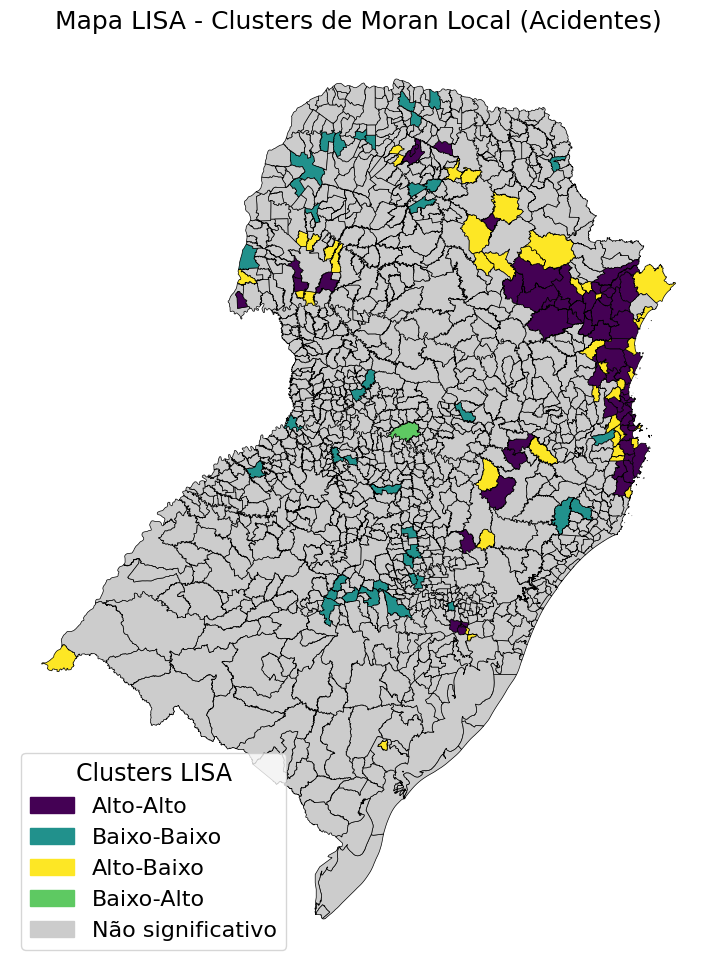
\includegraphics[width=.5\textwidth]{figures/3 - abordagem estatistica/1 - LISA.png}
\caption{LISA}
\label{fig:exampleFig4}
\end{figure}

Utilizando o dataset de radares foi criado uma nova coluna que delimita uma zona de influência de um radar. Conforme dispõe o art. 4º, § 7º da Resolução Contran nº 396/2011, a instalação de novos radares estáticos, móveis ou portáteis deve respeitar distâncias mínimas de 500 m em vias urbanas (ou rurais com características urbanas) e 2 km em vias rurais ou de trânsito rápido \cite{araujo2006}. Utilizando essa base, foi desenvolvido uma zona de influência de 500m em torno dos radares.

Com a definição da zona de influência de cada radar, foi verificado se os acidentes ocorriam dentro dessa área por meio de um join espacial. Para facilitar a análise, criou-se uma coluna booleana indicando a presença ou ausência de um radar próximo a cada acidente. Em seguida, foi necessário avaliar se o radar já estava ativo no momento do acidente. Para isso, a coluna de datas dos acidentes foi convertida para o formato datetime e comparada com a data de ativação do radar, gerando uma nova coluna booleana que indica se o radar estava ativo quando o acidente ocorreu.

Entre todos os acidentes, 19,37\% ocorreram próximos a algum radar. No entanto, ao considerar apenas os radares que já estavam ativos na data do acidente, esse percentual cai para 14,11\%.
No caso dos acidentes com vítimas fatais, 10,99\% aconteceram próximos a radares, mas, levando em conta apenas os que estavam ativos, o valor se reduz para 5,87\%.

Como o objetivo do projeto está em apontar pontos críticos nas rodovias federais, foi feito um filtro para retirar os acidentes que ocorreram próximos dos radares, deixando apenas os acidentes que aconteram fora do raio de atuação do radar. Após foi feito o agrupamento do DataFrame pelas colunas rodovia (br) e quilômetro (km), somando os valores da coluna mortos dentro de cada grupo. Dessa forma, foi gerado o total de mortos para cada combinação específica de rodovia e quilômetro.

Como os acidentes frequentemente ocorrem em locais muito próximos, foram definidas faixas de quilômetros para agrupar e representar melhor essas áreas de maior concentração. Neste projeto, utilizou-se um intervalo de 5 km, resultando em um DataFrame que apresenta a rodovia, a faixa correspondente, a quantidade de acidentes e o total de mortos.

Com base nesses dados, os acidentes foram organizados de acordo com o número de mortes, conforme mostrado na Figura ~\ref{fig:exampleFig5}. O destaque é para a faixa entre os quilômetros 0 e 5 da BR-277, que registrou 8 acidentes fatais. Em seguida aparecem a faixa 155–160 da BR-116, a faixa 45–50 da BR-470 e a faixa 80–85 da BR-470, cada uma com 6 acidentes fatais.

\begin{figure}[!htb]
\centering
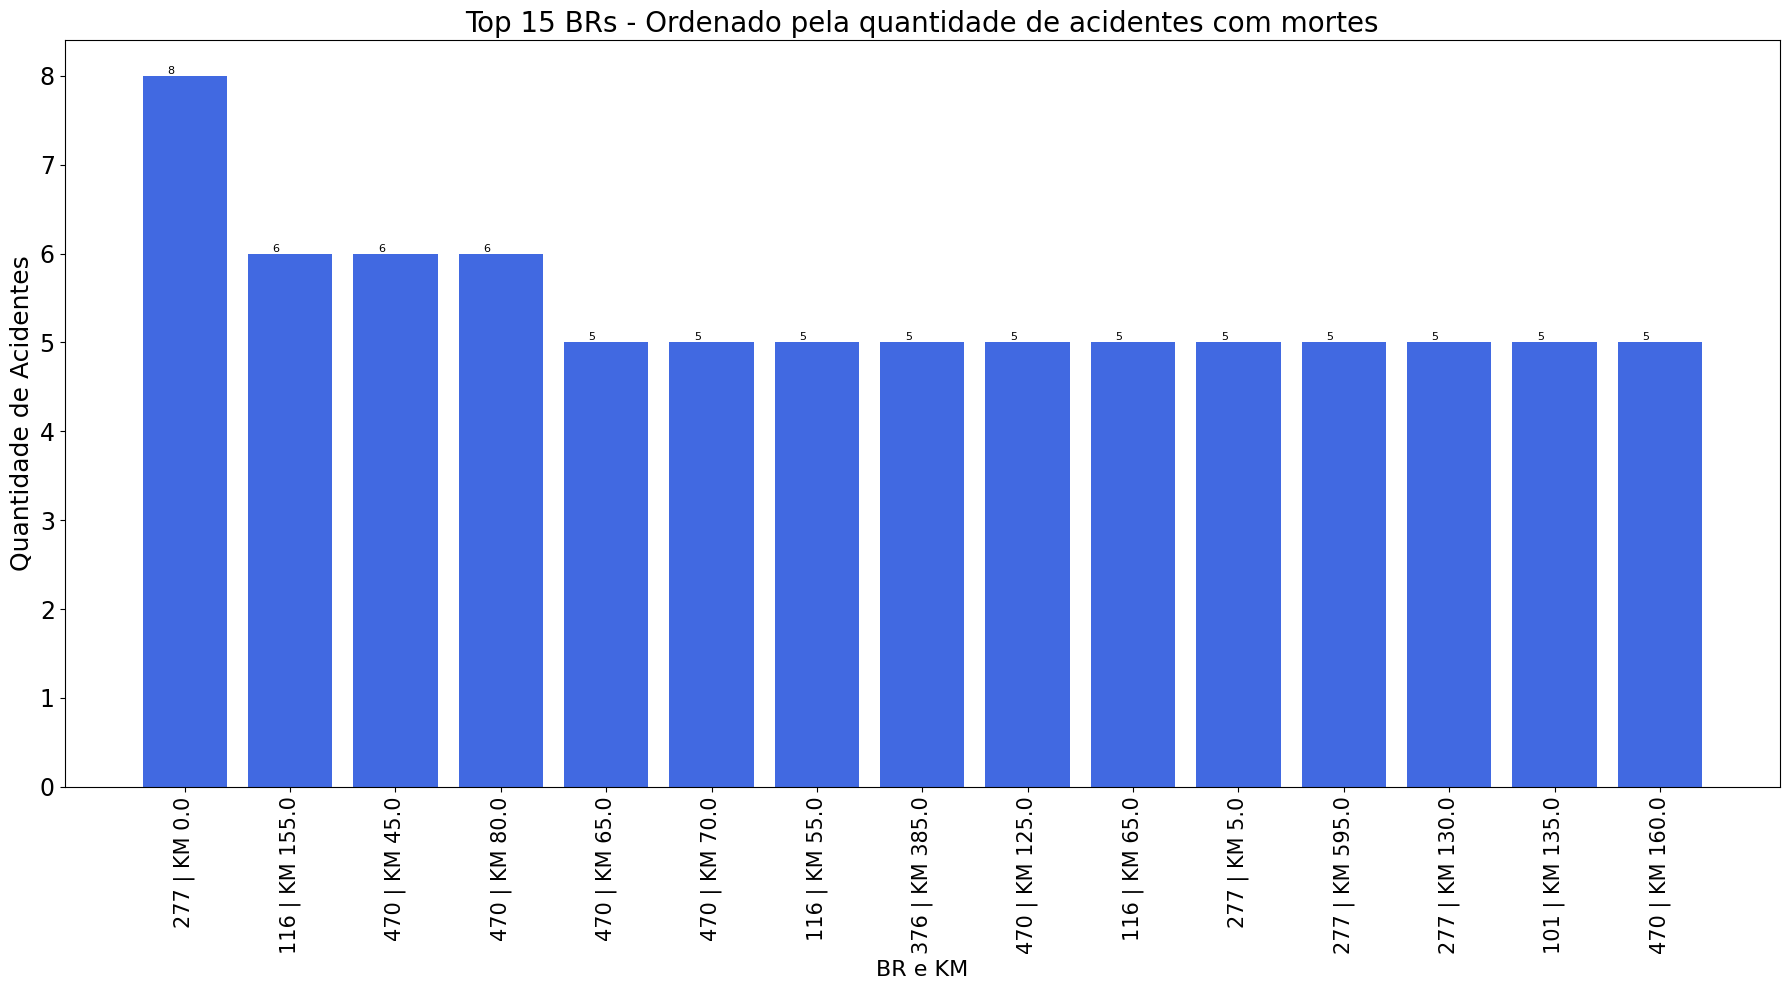
\includegraphics[width=1\textwidth]{figures/4 - abordagem radares/1 - top15 br acidentes com mortes.png}
\caption{Rodovias e quilometros com mais mortes}
\label{fig:exampleFig5}
\end{figure}

Considerando os acidentes totais (tanto com vítimas fatais como os sem vítimas fatais), o resultado pode ser visualizado na Figura ~\ref{fig:exampleFig6}, onde pode ser observado que a faixa de quilometros 135-140 da BR101 possui 37 acidentes, seguida da faixa 0-5 da BR277 e logo após a faixa 0-5 da BR376.

\begin{figure}[!htb]
\centering
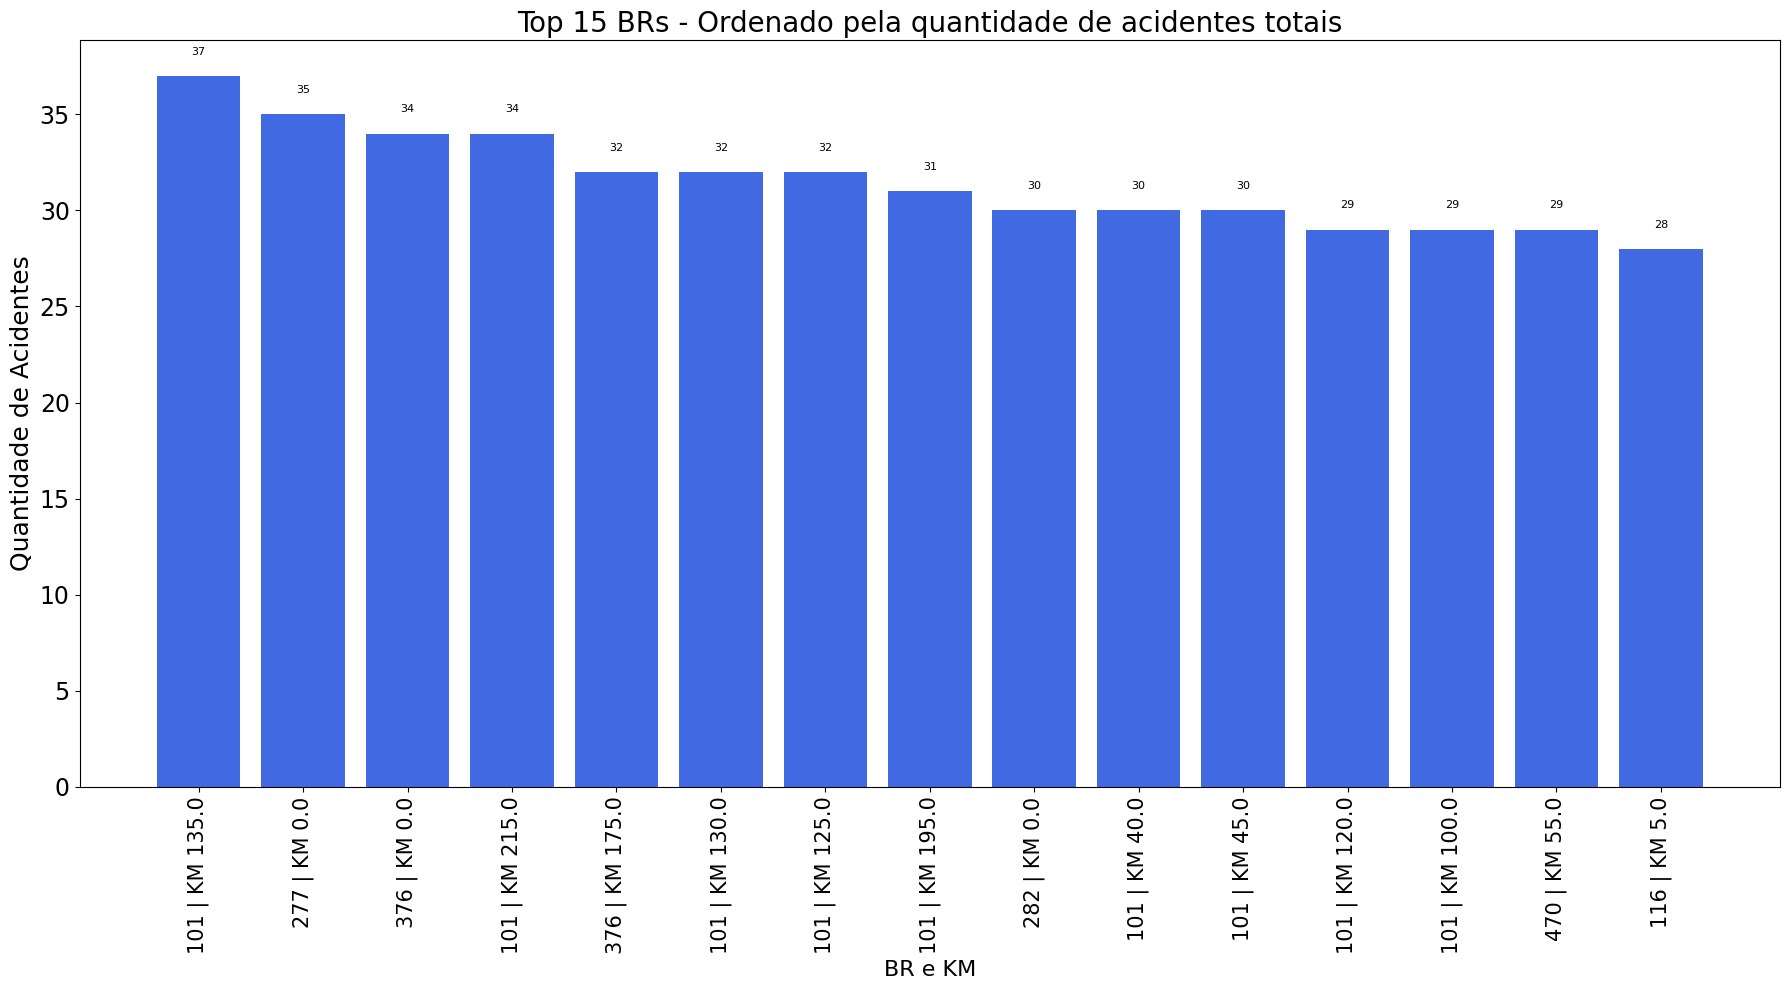
\includegraphics[width=1\textwidth]{figures/4 - abordagem radares/2 - top15 br acidentes totais.png}
\caption{Rodovias e quilometros com mais acidentes}
\label{fig:exampleFig6}
\end{figure}

%%%%%%%%%%%%%%%%%%%%%%%%%%%%%%%%%%%%%%%%%%%%%%%%%%%%%%%%%%%%%%%%%%%%%%
\section{Resultados}
%%%%%%%%%%%%%%%%%%%%%%%%%%%%%%%%%%%%%%%%%%%%%%%%%%%%%%%%%%%%%%%%%%%%%%



%%%%%%%%%%%%%%%%%%%%%%%%%%%%%%%%%%%%%%%%%%%%%%%%%%%%%%%%%%%%%%%%%%%%%%
\section{Conclusão}
%%%%%%%%%%%%%%%%%%%%%%%%%%%%%%%%%%%%%%%%%%%%%%%%%%%%%%%%%%%%%%%%%%%%%%

Diante da análise realizada, observa-se que a concentração de acidentes fatais está associada a trechos específicos de rodovias distantes da cobertura de radares. 
Nesse sentido, os pontos destacados na Figura \ref{fig:exampleFig5}, especialmente os quatro primeiros trechos, configuram-se como áreas prioritárias para a instalação de novos dispositivos de monitoramento. 
A inclusão estratégica desses pontos tem o potencial de gerar uma redução na taxa de mortalidade da região, dada sua relevância ao cenário nacional. 
Além disso, quando se considera a diminuição da taxa global de acidentes, os resultados evidenciados na Figura \ref{fig:exampleFig6} apontam para a BR-101 e a BR-376 como rodovias críticas, cuja elevada frequência de ocorrências reforça a necessidade de medidas preventivas adicionais. 

Portanto, a integração das análises de mortalidade e de volume de acidentes permite identificar trechos prioritários, orientando políticas públicas mais eficazes para a redução dos índices de sinistros nas rodovias federais brasileiras.

%%% Formato de figura
% \begin{figure}[ht]
% \centering
% \includegraphics[width=.5\textwidth]{fig1.jpg}
% \caption{A typical figure}
% \label{fig:exampleFig1}
% \end{figure}

\bibliographystyle{sbc}
\bibliography{sbc-template}

\end{document}
